%Hole Semantics: Semântica de Vãos? Semântica de Buracos? Semântica de Lacunas?


%\subsection{Considerações Iniciais}

\fixed{Solução fácil para eliminar o espaço: fim de uma subseção de considerações iniciais}
%
Desejamos associar a cada expressão de linguagem natural um significado formal, simbólico. Além disso, desejamos fazê-lo de modo algorítmico, que possa ser reproduzido por um computador. Portanto, um primeiro passo importante é encontrar um modo adequado de representar o significado, que satisfaça nossos objetivos lingüísticos, bem como que seja manipulável por nossas ferramentas computacionais.

A linguagem formal que utilizaremos para representar o significado de frases é \textit{lógica de primeira ordem}. \citet{Jurafsky:2009} apresentam como propriedades interessantes para representações: verificabilidade, não-ambigüidade, existência de uma forma canônica, capacidade de inferência, uso de variáveis e expressividade. Todas estas são possuídas pela lógica de primeira ordem, ao menos até certo ponto. \todo{argumentar, pegar referência} Além disso, é um sistema bem compreendido e bastante flexível.

\subsection{Lógica de Primeira Ordem}

Definiremos formalmente a sintaxe e a semântica da lógica de primeira ordem. A linguagem usada é definida a partir de um vocabulário. Um vocabulário consiste em três conjuntos de símbolos: um de predicados, um de funções e um de constantes. Cada um desses conjuntos é um conjunto de palavras, em que cada palavra é associada a um número, dito sua \textit{aridade}. No caso do conjunto de constantes, a aridade de cada elemento é $0$. \footnote{Mais a rigor, podemos dizer que são conjuntos de pares ordenados $(palavra,aridade)$.}

Assim, assumimos que possuímos o seguinte conjunto de símbolos:
\begin{enumerate}
\item 	Símbolos Lógicos:
		\begin{enumerate}
		\item parênteses: $($, $)$,
		\item conectivos: $\neg$, $\rightarrow$, $\land$, $\lor$
		\item quantificadores: $\forall$, $\exists$
		\item para variáveis: $x$, $y$, $z$, $\dots$ (um conjunto infinito delas)
		\item igualdade: $=$
		\end{enumerate}
\item	Símbolos não lógicos:
		\begin{enumerate}
		\item um conjunto de símbolos de predicados
		\item um conjunto de símbolos de constantes
		\item um conjunto de símbolos de funções
		\end{enumerate}
\end{enumerate}

\begin{defn}[Termo]
\begin{enumerate}
\item[]
\item Se $x$ é uma variável, $x$ é um termo.
\item Se $c$ é uma constante, $c$ é um termo.
\item Se $t_1$, \dots, $t_n$ são $n$ termos e $f$ é um símbolo de função de aridade $n$, então $f(t_1,\dots,f_n)$ é um termo.
\end{enumerate}
\end{defn}

\begin{defn}[Fórmula atômica]
\begin{enumerate}
\item []
\item Se $p$ é um predicado de aridade $n$ e $t_1$, \dots, $t_n$ são $n$ termos, então $p(t_1,\dots,t_n)$ é uma fórmula atômica.
\item Se $t_1$ e $t_2$ são termos, então $t_1 = t_2$ é uma fórmula atômica.
\end{enumerate}
\end{defn}

\begin{defn}[Fórmula]
\begin{enumerate}
\item[]
\item Se $\phi$ é uma fórmula atômica, então é uma fórmula.
\item Se $\phi$ e $\psi$ são fórmulas, então $\neg \phi$, $(\phi \rightarrow \psi)$, $(\phi \lor \psi)$ e $(\phi \land \psi)$ são fórmulas.
\item Se $x$ é uma variável e $\phi$ é uma fórmula, então $\forall x(\phi)$ e $\exists x(\phi)$ são fórmulas.
\end{enumerate}
\end{defn}

\begin{defn}[Modelo]
Um modelo é um par $(D,F)$ em que $D$, chamado \textit{domínio}, é um conjunto não vazio e $F$ é uma função, dita função de interpretação, tal que:
\begin{enumerate}
\item $F$ associa cada símbolo de constante do vocabulário a um elemento de $D$.
\item se $f$ é um símbolo de função de aridade $n$, $F$ associa $f$ a uma função $f^{F}: D^{n} \rightarrow D$.
\item se $p$ é um símbolo de predicado de aridade $n$, $F$ associa $p$ a um conjunto $p^{F} \subseteq D^{n}$.
\end{enumerate}
\end{defn}

\begin{defn}[Atribuição]
Uma (função de) atribuição $g$ em um modelo $(D,F)$ é uma função das variáveis no domínio $D$. Se $x$ for uma variável, uma atribuição $g'$ é dita uma $x$-variante quando, para toda variável $y$ distinta de $x$, $g'(y) = g(y)$.
\end{defn}

\begin{defn}[Interpretação]
Seja $t$ um termo, $M = (D,F)$ um modelo e $g$ uma atribuição em M. A interpretação $I_F^g$ de $t$ com respeito a $M$ e $g$ é definida indutivamente por:
\begin{enumerate}
\item se $t$ é uma variável, $I_F^g(t) = g(t)$.
\item se $t$ é uma constante, $I_F^g(t) = F(t)$.
\item se $t$ é $f(t_1,\dots,t_n)$, onde $f$ é um símbolo de função e $t_1$, \dots, $t_n$ são termos, então $I_F^g(t) = f^{F}(I_F^g(t_1), \dots, I_F^g(t_n))$.
\end{enumerate}
\end{defn}

\begin{defn}[Satisfação]
Sejam $M = (D,F)$ um modelo, $g$ uma atribuição em M e $\phi$ e $\psi$ fórmulas. Então, a relação de satisfabilidade $\models$ é definida indutivamente:
\begin{enumerate}
\item $M,g \models p(t_1,\dots,t_n)$ se e somente se $(I_F^g(t_1), \dots, I_F^g(t_n)) \in F(p)$ , em que $p$ é um símbolo de predicado e $t_1$, \dots, $t_n$ são termos.
\item $M,g \models \neg \phi$ se e somente se não for verdade que $M, g \models \phi$.
\item $M,g \models \phi \land \psi$ se e somente se $M, g \models \phi$ e $M, g \models \psi$.
\item $M,g \models \phi \lor \psi$ se e somente se $M, g \models \phi$ ou $M, g \models \psi$.
\item $M,g \models \phi \rightarrow \psi$ se e somente se não for o caso tanto que $M,g \models \phi$ quanto que $M,g \not \models \psi$.
\item $M,g \models \exists x (\phi)$ se e somente se existir uma $x$-variante $g'$ de $g$ tal que $M,g' \models \phi$.
\item $M,g \models \forall x (\phi)$ se e somente se para toda $x$-variante $g'$ de $g$, $M,g' \models \phi$.
\end{enumerate}
\end{defn}

Para mais detalhes a respeito da lógica de primeira ordem, recomendamos o livro de \citet{enderton}.

\update
\todo{escrever texto}

%Também uma interessante propriedade da lógica de primeira ordem é sua relativa intuitividade. Bastando explicar o que significam os símbolos conectivos (como $\land$ (significando \expr{e}) e $\rightarrow$ (significando \expr{se \dots então \dots})), bem como os quantificadores ($\forall$ (\expr{para todo})  e $\exists$ (\expr{existe}), uma expressão formal em lógica é compreensível . %\todo{é verdade?}

\subsection{Sintaxe e representação de expressões}

Ainda que tenhamos escolhido a lógica de primeira ordem para ser a linguagem das representações semânticas para frases, isto não nos informa qual deve ser a representação semântica de palavras e expressões menores. Fórmulas desta lógica definem sentenças completas (no máximo, abertas à interpretação de variáveis livres). Talvez algumas possibilidades poderiam ser feitas através de termos, mas não está de todo claro qual seria o significado de uma expressão como \expreng{to run} (\expr{correr}) ou \expreng{that walks} (\expr{que anda}).


Presente já no desenvolvimento inicial da semântica formal, adotaremos o \textit{Princípio da Composicionalidade}, usualmente atribuído a Gottlob Frege \cite[p.~94]{BlackburnBos:2005}.
%
\updated{A ambigüidade anterior era se o pressuposto era original ou já anterior, correto? Assim fica melhor?}
%
Segundo o mesmo, o significado de expressões complexas é função das expressões mais simples que a compõem. Em um exemplo como \expreng{Caim kills Abel}, isto nos informa que o significado desta frase depende do significado de \expreng{Caim}, \expreng{kills} e \expreng{Abel}. Entretanto, isto não nos diz como funciona esta dependência, ou a função que leva o significado das expressões simples ao da expressão complexa.

Por exemplo, podemos entender que o significado de \expreng{kills} é o predicado binário \code{kill(\dots , \dots)}, onde convencionamos que o primeiro argumento é o agressor (isto é, aquele que mata) e o segundo argumento é a vítima (aquele que é morto). Também podemos entender os significados de \expreng{Caim} e \expreng{Abel} como as constantes \code{caim} e \code{abel}, respectivamente. Assim, apesar de \code{kill(abel,caim)} ser formada com o significado destes três termos, respeitando a composicionalidade, esta não é a expressão que queremos, e sim \code{kill(caim,abel)}.

O que nos falta é a \textit{sintaxe}. A sintaxe é o conjunto de regras e processos que organizam a estrutura de frases \citep[p.~2]{vanEijck:2010}. Assim, as palavras em uma frase existem em relação a uma certa estrutura, que é essencial para capturar o significado. No inglês, com a estrutura usual de \textit{Sujeito - Verbo - Predicado}, entendemos que \expreng{Caim kills Abel} significa \code{kill(caim,abel)}, e não \code{kill(abel,caim)}.

Para nos atermos mais nos desenvolvimentos semânticos, 
%
\updated{Não me parece exagero dizer que o foco não é na sintaxe. O próprio Bos afirma que uma desvantagem de tal abordagem é que o leitor não aprenderá nada interessante sobre sintaxe. De todo modo, alterei. O que acha?}
%
utilizamos uma sintaxe simples: a gramática é implementada pelo mecanismo de Gramática de Cláusulas Definidas (\textit{Definite Clause Grammar} - DCG). A análise sintática é feita na forma de uma árvore cujos nós que são folhas são categorias sintáticas básicas (tais como sujeito (\teng{noun}), verbo transitivo (\teng{transitive verb}) e quantificador (\teng{quantifier}, considerado caso particular de \teng{determiner}). Já os nós que não são folhas representam categorias sintáticas complexas (tais como sintagma nominal (\teng{noun phrase}) ou sintagma verbal (\teng{verb phrase}) \cite[p.~58]{BlackburnBos:2005}. %Fossem apenas as classes gramaticais, seria uma Gramática Livre de Contexto. Porém, a Gramática de Cláusulas Definidas aceita o uso de algumas restrições, indo além de tal formalismo,como restrições de concordância de número. %Talvez mesmo assim seja possível converter em uma Context Free Grammar (CFG).

Um exemplo de tal árvore, para a frase \expreng{\teng{Caim kills Abel}}, seria:

\Tree [.{\teng{Caim kills Abel} (\teng{Sentence}) } 
[.{\teng{Caim} (\teng{NP})} {\teng{Caim} (\teng{PN})} ]
[.{\teng{kills Abel} (\teng{VP})}
{\teng{kills} (\teng{TV})} [.{\teng{Abel} (\teng{NP})} {\teng{Abel} (\teng{PN})} ] ]
] \\

Aqui, temos as classes sintáticas:\\
\teng{NP} -- \teng{noun phrase} (sintagma nominal)\\
\teng{PN} -- \teng{proper noun} (nome próprio)\\
\teng{VP} -- \teng{verb phrase} (sintagma verbal)\\
\teng{TV} -- \teng{transitive verb} (verbo transitivo)

A decomposição parece lingüisticamente razoável, bem como útil para a compreensão do significado. Resta saber, assim, como podemos elaborar a construção da semântica de uma frase completa a partir de tal análise sintática e dos significados dos termos mais elementares. Portanto, devemos construir nossa gramática.

%Essa idéia nos seguirá pelo restante do trabalho, permitindo separar nossas análises, bem como nossos códigos, pelo seguinte norte: a sintaxe da nossa linguagem natural objeto pode ser separada em léxico -- a análise de palavras ou expressões em si, como unidades básicas -- e em regras gramaticais -- a análise de como as classes sintáticas se compõem para formar novas, bem como outras relações de concordância (como concordância de gênero ou de número). Já a semântica também pode ser tratada a nível de léxico -- em que cada classe sintática básica terá um modelo próprio de interpretação semântica -- bem como a nível de regras -- em que a semântica de uma expressão complexa será formada por uma forma de composição entre as semânticas das expressões que a constituem.

\subsection{Arquitetura da Gramática} \label{sec:arquitetura}

	\citet[p.~86]{BlackburnBos:2005} apontam três princípios a serem observados na construção da gramática: modularidade -- divisão da gramática em componentes com finalidades bem definidas e que interagem de modo transparente --, extensibilidade -- ser fácil de complementá-la -- e reusabilidade -- capacidade de reaproveitar grandes partes da gramática, mesmo alterando as representações semânticas.
	
	Para seguí-los, o método usado foi dividir a gramática segundo dois critérios: se o componente trata do léxico ou de regras gramaticais (isto é, combinando expressões para criar outras maiores) e se é sintático ou semântico. Assim, um dos componentes da gramática é um léxico que enumera as palavras e expressões aceitas, afirmando determinadas propriedades. Um segundo trata da semântica dos léxicos, isto é, da representação semântica dada a palavras individualmente ou expressões básicas (aqui, isto é principalmente feito se utilizando da classificação sintática, isto é, a classe sintática e a palavra em si determinam a semântica). Um terceiro item trata das regras da sintaxe, isto é, da classificação sintática de expressões complexas a partir da classificação de termos menos (incluindo aspectos como concordância de gênero ou número). Ademais, um quarto componente trata das regras semânticas, isto é, como combinar o significado de expressões menores para formar o significado de expressões maiores. Por fim, utilizamos uma quinta parte que se utiliza de todas as anteriores para fazer a relação entre o texto recebido e a representação semântica desejada. Um exemplo pode ser visto na tabela \ref{curt-gramatica}, tratando do exemplo da representação semântica mais simples, a do cálculo lambda, que veremos a seguir.
	
	\todo[color=yellow,inline]{De fato é assim que o código será organizado, mas o lambda.pl é apenas o mais simples, então não deixa de ser um exemplo. O mecanismo completo não usará o lambda.pl. Mais detalhes do projeto, link e deixar o código livre eu deixei para o capítulo de Curt, ou então posso colocar na introdução}
	
	\begin{table}[h]
		\centering
		\begin{tabular}{|c|c|c|}
				\hline \textsc{lambda.pl} & sintaxe & semântica \\ 
				\hline léxico & \textsc{englishLexicon.pl} & \textsc{semLexLambda.pl} \\ 
				\hline gramática & \textsc{englishGrammar.pl} & \textsc{semRulesLambda.pl} \\ 
				\hline 
		\end{tabular}
		\caption{Gramática para semântica lambda}
		\label{curt-gramatica}
	\end{table}
		 
	Ao alterarmos a representação semântica, de fato nossas principais alterações estarão nos componentes semânticos.
	
	Seguiremos o desenvolvimento de \citet{BlackburnBos:2005} dos diferentes módulos semânticos. Um primeiro modelo ilustrará um formalismo fundamental para composição de significados, o cálculo lambda. Para que a relação deste formalismo com o significado seja isolada de outros mecanismos usados posteriormente, ele será apresentado isoladamente em um primeiro lugar. Além disto, neste modelo inicial cada frase será associada a exatamente uma fórmula em lógica de primeira ordem, enquanto palavras e expressões menores serão associadas a um outro tipo de fórmula - fórmulas do cálculo lambda.
	
	A seguir, para sanar alguns de seus problemas, um passo de abstração será tomado. Expressões e frases não necessariamente serão associadas a exatamente uma fórmula, mas sim a um conjunto delas. Isto são as ditas \textit{representações subespecificadas}. Há uma variedade de métodos para representações subespecificadas e aqui veremos três, mas exploraremos essencialmente representantes de dois grupos. Os dois grupos serão vistos para o estudo de abordagens distintas para o problema da subespecificação. \citep[p.~150--153]{BlackburnBos:2005}
	
	O primeiro método será o de armazenamentos, a ser introduzido em sua versão mais simples, o armazenamento de Cooper. Veremos como isto é uma melhora, mas ainda não o bastante. Após isto, ele será aprimorado pelo armazenamento de Keller.
	
	Do segundo grupo, veremos a \teng{hole semantics}, um formalismo essencialmente diferente, baseado em restrições, devido a \citet{HoleSem}.

	\todo[color=yellow,inline]{atualizei com uma descrição das diferentes técnicas, bem como dizendo que seguiremos as diferentes técnicas}

\subsection{Cálculo Lambda}

Para realizar um método sistemático de composição dos significados, é introduzido o formalismo do \textit{cálculo lambda}. Aqui, ele será uma extensão da linguagem da lógica de primeira ordem. Dois símbolos novos serão introduzidos: o símbolo de abstração \expr{$\lambda$} e o de aplicação \expr{$@$}.

O símbolo \expr{$\lambda$} será um operador sobre variáveis, permitindo a ``captura'' das mesmas, do mesmo modo a que um quantificador (como \expr{$\forall$}). Por exemplo, sendo \code{man(x)} uma fórmula de primeira ordem, \code{\lambda x.man(x)} é uma fórmula do nosso cálculo lambda, em que a variável $x$ está capturada pelo operador $\lambda$; alternativamente, $\lambda x.$ está \textsl{abstraindo sobre} $x$. 

Por sua vez, o símbolo \expr{$@$}, que conecta duas fórmulas de cálculo lambda, representa uma \textit{aplicação}. Assim, se $F$ e $A$ são duas fórmulas de cálculo lambda, $F@A$ é também uma fórmula de cálculo lambda, chamada uma \textit{aplicação funcional} de $F$ em $A$, ou uma aplicação na qual $F$ é um \textsl{funtor} e $A$ é o \textsl{argumento}. Por exemplo, em \code{(\lambda x. man(x))@john}, o funtor é \code{\lambda x. man(x)} e o argumento é \code{john}.

Uma expressão de aplicação funcional representa o comando de aplicar o argumento no funtor, que usualmente será prefixado por uma abstração. A interpretação desse comando é: retire o prefixo de abstração do funtor e, em toda ocorrência da variável abstraída, a substitua pelo argumento da aplicação. Por exemplo, em \code{(\lambda x. man(x))@john}, o funtor é \code{\lambda x. man(x)} e a interpretação do comando é de retirar o prefixo \code{\lambda x.} e substituir toda ocorrência de \code{x} no funtor pelo argumento \code{john}, o que produz o resultado de \code{man(john)}. Transformar uma aplicação em sua fórmula resultante após o processo de aplicação é uma operação chamada de \textit{$\beta$-redução}, \textit{$\beta$-conversão} ou \textit{$\lambda$-conversão} \citep[p.~67]{BlackburnBos:2005}.

Destacamos que aplicações podem ser subfórmulas de outras fórmulas, com a $\beta$-redução da fórmula maior sendo a $\beta$-redução de suas subfórmulas, bem como que não é necessário ser um termo ou uma variável para ser um argumento de uma aplicação. Ademais, convencionaremos que o operador \code{@} possui precedência em relação ao operador \code{\lambda}. Outra convenção será a de que o operador \code{@} se associa à direita. Deste modo, devemos ler $\lambda P. P@z$ como $\lambda P.(P@z)$, enquanto $(\lambda P. \lambda Q. P)@x@y$ deve ser lido como $((\lambda P. \lambda Q. P)@x)@y$. \updated{Precedência. O Bos não explicita o critério dele, então elegi esse.}

Veja este exemplo:
É bem formada a fórmula $(\lambda P. P@mia)@(\lambda x.woman(x))$. Em uma primeira etapa de $\beta$-redução, chegamos à fórmula $(\lambda x.woman(x))@mia$ e aí, mais uma vez realizando a operação, chegamos à sua $\beta$-redução final $woman(mia)$.

Um cuidado a se ter é que pode ser necessário trocar o símbolo das variáveis em uma aplicação. É suficiente trocar todas as variáveis ligadas (isto é, capturadas por um operador) do funtor por variáveis novas, não utilizadas até então. A operação de substituir todas as variáveis ligadas por outras é chamada de \textit{$\alpha$-conversão}, enquanto se uma fórmula pode ser gerada através de $\alpha$-conversão de outra, as duas fórmulas são ditas \textit{$\alpha$-equivalentes}. Para um exemplo em que não realizar a $\alpha$-conversão antes de uma $\beta$-conversão pode gerar problemas, basta realizar a $\beta$-conversão da seguinte expressão: $(\lambda x .\exists y. not\_equal(x,y)) @ y$. O resultado incorreto seria $\exists y. not\_equal(y,y)$, enquanto o resultado adequado seria $\exists y. not\_equal(z,y)$.

Desse modo, temos o cálculo lambda como uma ``linguagem de cola'', permitindo fazer composições de expressões até gerar verdadeiras expressões de primeira ordem. A abordagem então é criar, de algum modo, a representação semântica a nível de léxico (isto é, a nível de classes sintáticas básicas), bem como montar a representação semântica a nível da gramática, pela composição de termos mais simples, de algum modo compatível com a semântica a nível lexical. Vejamos alguns exemplos:

Para nomes próprios (\teng{proper names}), a semântica é: \code{\lambda u. u @ symbol}, onde \code{symbol} representa o símbolo do nome próprio (por exemplo, \code{john}).

Por sua vez, para verbos transitivos temos a semântica \code{\lambda k. \lambda y. k@(\lambda x. symbol(y,x))}, onde mais uma vez \code{symbol} reprenta o símbolo específico da palavra (por exemplo, \code{kill}).

Pensemos agora no sintagma verbal (\teng{verb phrase}) \expreng{kills Abel}. Um modo natural de pensar na composição é, sendo $A$ a expressão semântica de \expr{kill} e $B$, a de \expr{Abel}, realizar a aplicação $A@B$. Com efeito, fazendo isso teríamos:
\begin{align*}
&(\lambda k. \lambda y. k@(\lambda x. kill(y,x))) @ \lambda u. u@abel \\
& \lambda y. ((\lambda u. u@abel)@(\lambda x. kill(y,x))) \\
& \lambda y. (\lambda x.kill(y,x)@abel) \\
& \lambda y. kill(y,abel)
\end{align*}

Agora, podemos juntar o sintagma nominal (e também nome próprio) \expreng{Caim} e o sintagma verbal \expreng{kills Abel}, aplicando a semântica do segundo na do primeiro, de onde teríamos:
\begin{align*}
&(\lambda u. u@caim)@(\lambda y.kill(y,abel)) \\
& (\lambda y. kill(y,abel))@caim \\
& kill(caim,abel)
\end{align*}

Assim, chegamos a uma representação da frase \expreng{Caim kills Abel} que é uma expressão de lógica de primeira ordem, utilizando o cálculo lambda como ferramenta para composição sistemática do sentido de expressões menores.

\subsubsection{Dificuldades -- Ambigüidades de Escopo}
Apesar deste método produzir resultados interessantes, ele não é suficiente. Uma característica particular é que, do modo que realizamos, cada decomposição sintática está associada a apenas uma possibilidade semântica. Isto não quer dizer que o modelo até então não consegue tratar de ambigüidades.

Em primeiro lugar, as ambigüidades lexicais podem ser tratadas colocando em nosso sistema todos os sentidos possíveis de determinada expressão. Assim, homógrafos (palavras com a mesma grafia mas significados distintos) podem ser considerados como entradas distintas em nosso banco de dados da semântica lexical. Devido ao mecanismo de \teng{\textit{backtracking}} da linguagem Prolog, todas as possibilidades são facilmente geradas, fazendo com que a simples adição da entrada lexical é suficiente para que este tipo de ambigüidade seja capturado. De fato, é disto que nos beneficiamos em nossa integração com a Wordnet, explorada na seção \ref{sec:wordnet}.

Em segundo lugar, ambigüidades por diferentes possibilidades de decomposição sintática de uma mesma frase também podem ser tratadas pelo modelo até então. Novamente, a implementação se beneficia do mecanismo de \teng{\textit{backtracking}} do Prolog, de modo que diferentes decomposições sintáticas e seus significados associados podem ser gerados sucessivamente.

\todo[inline]{Checar ambigüidades sintáticas.... Funciona mesmo? Exemplo?}

Entretanto, podemos apontar um tipo de ambigüidade que, até então, nosso modelo é incapaz de tratar: as ditas \textit{ambigüidades de escopo} \citep[p.~105-109]{BlackburnBos:2005}. As ambigüidades de escopo são melhor explicadas através de exemplos.

Analisemos a frase: 
\begin{align*}
\text{\expreng{Every man loves a woman.}}
\end{align*}%ocorrem quando há dúvidas a respeito da precedência, ou da ``captura'', de um conteúdo semântico em relação a outros.

Esta frase parece ter duas interpretações possíveis: na primeira, para cada homem existe uma mulher amada por aquele. Possivelmente, são mulheres distintas. Já na segunda leitura, existe uma mulher específica que é amada por todos os homens.

\update Essa dúvida parece ser gerada pelo \textit{escopo} dos quantificadores \expreng{every} e \expreng{a}. Caso o quantificador \expreng{every} seja \textit{mais externo} (ou \textit{\teng{out-scoping}}) ao quantificador \expreng{a}, então teremos a primeira leitura. Neste caso, também dizemos que o quantificador \expreng{every} tem \textit{escopo sobre} o quantificador \expreng{a}. Por outro lado, caso o quantificador \expreng{a} tenha escopo sobre o quantificador \expreng{every}, a leitura será a segunda. Isto é, em nossa semântica, a primeira leitura seria representada por

\begin{align*}
\forall x (man(x) \rightarrow \exists y (woman(y) \land love(x,y)))
\end{align*}

O quantificador existencial está ``dentro do alcance'' do quantificador universal. Já na segunda leitura ocorreria o contrário, sendo:

\begin{align*}
\exists y (woman(y) \land \forall x(man(x) \rightarrow love(x,y)))
\end{align*}

Perceba que, ao que parece, as ambigüidades de escopo não são geradas por, realmente, análises sintáticas distintas, mas sim por uma dificuldade de atribuição de significado à uma decomposição sintática em particular.

Com efeito, na gramática que utilizamos, esta frase seria decomposta sintaticamente segundo a figura \ref{tree:syntax}. Para as duas interpretações, a decomposição sintática é a mesma, mostrando que o problema é semântico.

\begin{figure}
%\begin{center}
\begin{tikzpicture}
%\tikzset{level distance=40pt}
\tikzset{frontier/.style={distance from root=100pt}}
\Tree [.{\teng{Every man loves a woman} (\teng{Sentence}) } 
[.{\teng{Every man} (\teng{NP})} {\teng{Every} (\teng{Determiner})} {\teng{man} (\teng{Noun})} ]
[.{\teng{loves a woman} (\teng{VP})}
{\teng{loves} (\teng{TV})} [.{\teng{a woman} (\teng{NP})} {\teng{a} (\teng{Determiner})} {\teng{woman} (\teng{Noun})} ] ]
]
\end{tikzpicture}
%\end{center}
\caption{Árvore Sintática}
\label{tree:syntax}
\end{figure}

Que o nosso sistema atual não é capaz de representar esse tipo de ambigüidade pode ser visto pelo fato de que a representação semântica é única, dados o sentido dos termos mais simples e a decomposição sintática. Precisamos, assim, aprimorar o modelo.

Para termos um olhar em direção à solução, podemos notar que a ocorrência de quantificadores gera seus problemas na função sintática de sintagma nominal (\teng{noun phrase}), pois a combinação quantificador e substantivo (\teng{determiner + noun}) ocorre apenas nela. Isso sugere que alteremos o modo pelo qual tratamos a semântica dos sintagmas nominais com quantificadores.

\subsection{Armazenamento de Cooper}

Para o problema das ambigüidades de escopo, a solução computacional proposta é o uso de \textit{armazenamentos}. Nesta abordagem, a representação semântica de cada expressão deixa de ser a de uma simples fórmula em cálculo lambda, para ser a de uma representação de múltiplas formas possíveis.

Em particular, começaremos com o \textit{armazenamento de Cooper}. Esta é uma técnica desenvolvida por Robin Cooper para lidar com ambigüidades de escopo de quantificadores \cite[p.~113]{BlackburnBos:2005}. Intuitivamente, a idéia está em adicionar a possibilidade de substituir uma representação mais detalhada de um sintagma nominal por uma nova variável e ``armazenar'' a representação completa deste sintagma nominal para uso posterior. Ao fim, as representações podem ser ``resgatadas'' do armazenamento, em qualquer ordem. Ao se ``resgatar'' uma representação após alguma outra, o quantificador do sintagma nominal resgatado posteriormente poderá ter escopo mais externo do que um quantificador da representação ``resgatada'' anteriormente. Desse modo, ao se possibilitar os ``resgates'' em ordens distintas, diferentes representações são formadas.

Agora cada expressão (isto é, cada nó da árvore de análise sintática (\teng{parse})) é associada a uma $n$-upla chamada ``armazenamento''. O primeiro elemento do armazenamento será uma fórmula de cálculo lambda, bem como antes. É uma representação ``nuclear'' da expressão. Com efeito, chamaremos este elemento de \textit{núcleo} do armazenamento. Por sua vez, os outros elementos da $n$-upla serão pares $(\beta, i)$, em que $\beta$ é uma representação semântica para um sintagma nominal e $i$ é um indice para este sintagma. Estes pares são denominados \textit{operadores de ligação indexados} (\teng{indexed binding operators}).

Com mais detalhes, \textit{a priori} as representações não diferem muito de como eram. Os nós das folhas, não sendo nenhum um sintagma nominal quantificado, são análogos ao modo anterior, sendo armazenamentos com apenas uma entrada. Já um nó não-terminal pode ter sua representação montada de um modo ``usual'': ele tem como núcleo uma combinação dos núcleos de cada um de seus filhos na árvore; isto é, é a combinação dos núcleos dos armazenamentos dos termos que compõem a expressão mais complexa. Esta combinação é exatamente do mesmo modo como era feito até então. O restante do armazenamento do nó não-terminal é a justaposição (\teng{append}) do restante dos armazenamentos de cada um dos termos filhos. Em suma: quando a expressão é composta por outras na análise sintática, tudo ocorre de modo análogo a como ocorria na representação ``pura'' por cálculo lambda, preservando os operadores de ligação indexados de todas as sub-expressões que compõem a expressão maior.

Caso o nó não-terminal não seja um sintagma nominal quantificado, a represnetação ``usual'' é a sua única possível. Entretanto, o processo possui uma diferença quando o nó não-terminal é um sintagma nominal quantificado. Além da composição ``usual'' para outros nós, há uma segunda representação possível. Isso merece ser destacado:

\begin{oframed}\textbf{Armazenagem (Cooper)}\\
Seja o armazenamento $\langle\phi, (\beta, j), \dots, (\beta', k)\rangle$ a representação semântica ``usual'' para um sintagma nominal quantificado. O armazenamento $\langle\lambda u.(u@z_i), (\phi, i), (\beta, j), \dots, (\beta', k)\rangle $, onde $i$ é um índice único\footnotemark também é uma representação para este sintagma nominal quantificado.
\end{oframed}
\footnotetext{{isto é, não utilizado até então}}

Isto significa que sintagmas nominais quantificados podem ter suas representações montadas de dois modos. Neste ponto, nosso algoritmo terá uma escolha de aplicar ou não a regra de armazenagem. Ao se desejar saber a representação de uma frase em específico, esperaremos que nosso sistema nos retorne todas as representações possíveis. Perceba também que a regra não é recursiva. Há apenas duas opções: manter a representação ``usual'' ou realizar a operação de armazenagem.

Após todo este processo, teremos uma frase cuja representação é um armazenamento. É necessário lidar com isto de algum modo, pois o que desejamos é que uma frase possa ser representada por expressões de lógica de primeira ordem, não por um armazenamento. Aqui é que poderemos ``resgatar'' nossos operadores de ligação indexado, que foram previamente armazenados. Para isso, usaremos a seguinte regra de resgate:

\begin{oframed} \textbf{Resgate (Cooper)}\\
Sejam $\sigma_1$ e $\sigma_2$ duas seqüências (possivelmente vazias) de operadores de ligação. Se o armazenamento $\langle\phi, \sigma_1, (\beta, i), \sigma_2\rangle$ a uma frase (\teng{sentence}), então o armazenamento $\langle\beta @ \lambda z_i . \phi , \sigma_1, \sigma_2 \rangle$ também é associado a esta frase.
\end{oframed}

Um armazenamento composto apenas por um núcleo, após sucessivas aplicações da regra de resgate, será uma fórmula bem formada de primeira ordem, como desejávamos.

Para visualizarmos este processo, vamos para o exemplo da figura \ref{tree:syntax}, a árvore de análise sintática para a frase \expreng{Every man loves a woman}. Construindo os significados a partir das folhas e subindo, uma das possíveis árvores que podemos alcançar está na figura \ref{tree:cooper}.

\begin{figure}
\begin{center}
\begin{tikzpicture}
%\scriptsize
\footnotesize
%\small
\tikzset{level distance=100pt,align=center, sibling distance = 0pt}
\tikzset{frontier/.style={distance from root=300pt}}
%\tikzset{level 1/.style={level distance=36pt}}
%\tikzset{level 2+/.style={sibling distance=1pt}}
%\tikzset{level 3+/.style={level distance=28pt}}
\Tree [.{\teng{Every man loves a woman} (\teng{Sentence}) \\ $\langle love(z_1,z_2), $\\$ (\lambda q. \forall x(man(x) \rightarrow q@x), 1),$\\$ (\lambda q. \exists x(woman(x) \land q@x),2) \rangle$ } 
[.{\teng{Every man} (\teng{NP}) \\$\langle \lambda u . u@z_1 ,$\\$ (\lambda q. \forall x(man(x) \rightarrow q@x), 1) \rangle$} {\teng{Every} (\teng{Determiner}) \\ $\langle \lambda p . \lambda q. \forall x(p@x \rightarrow q@x) \rangle$} {\teng{man} (\teng{Noun}) \\ $\langle \lambda x. man(x) \rangle$} ]
[.{\teng{loves a woman} (\teng{VP}) \\ $\langle \lambda x. love(x,z_2),$\\$ (\lambda q. \exists x(woman(x) \land q@x),2) \rangle$}
{\teng{loves} (\teng{TV}) \\ $\langle \lambda k. \lambda x. k @ (\lambda y. love(x,y)) \rangle$} [.{\teng{a woman} (\teng{NP}) \\ $\langle \lambda u. u@z_2 ,$\\$ (\lambda q. \exists x(woman(x) \land q@x),2) \rangle$} {\teng{a} (\teng{Determiner}) \\ $\langle \lambda p. \lambda q. \exists x (p@x \land q@x) \rangle$} {\teng{woman} (\teng{Noun}) \\ $\langle \lambda x. woman(x) \rangle$} ] ]
]
\end{tikzpicture}
\end{center}
\normalsize
\caption{Semântica de Cooper}
\label{tree:cooper}
\end{figure}

Agora, o que resta é converter o armazenamento representativo da frase completa nas possíveis fórmulas de primeira ordem através da operação de resgate. 

\begin{flalign*}
 \text{Inicialmente:} \\
 \langle love(z_1,z_2),& \\ &(\lambda q. \forall x(man(x) \rightarrow q@x), 1),  (\lambda q. \exists x(woman(x) \land q@x),2) \rangle \\
 \text{Resgatando o operador de ligação 1:}  \\
 \langle \lambda q. \forall x(man(x) \rightarrow q@x) &@ (\lambda z_1 . love(z_1,z_2)),  \\&(\lambda q. \exists x(woman(x) \land q@x),2)\rangle \\
 \beta\text{-convertendo:} \\
 \langle \forall x (man(x) \rightarrow love(x,z_2)), &\\&(\lambda q. \exists x(woman(x) \land q@x),2)\rangle \\
 \text{Resgatando o operador de ligação 2:} \\
 \langle (\lambda q. \exists x(woman(x) \land q@x))@&(\forall x (man(x) \rightarrow love(x,z_2))) \rangle  \\
 \alpha\text{-convertendo e }  \beta\text{-convertendo:} \\
 \langle \exists x (woman(x) \land \forall y(man(y) &\rightarrow love(y,x))) \rangle  \\
\end{flalign*}

Assim, chegamos a uma das duas interpretações: a de que todos os homens amam uma mesma mulher. Se resgatarmos o operador de ligação 2 e só depois resgatarmos o operador de ligação 1, teremos a outra leitura: $\forall y(man(y) \rightarrow \exists x (woman (x) \land love(y,x)))$, isto é, para cada homem, existe alguma mulher tal que ele a ame.

Portanto, desenvolvemos um método sistemático que pode capturar as ambigüidades de escopo, produzindo as leituras possíveis. O que nos resta agora é a pergunta: será que nosso método é de fato capaz de capturar todas as ambigüidades de escopo? Infelizmente, iremos apontar duas frases nas quais o método não é suficiente. \fixed{De fato não estava nada claro! Retirei a afirmação.}

\subsubsection{Dificuldades}

A primeira frase é: \expreng{Every criminal with a gun is dangerous.} Aplicando nosso método, teremos os seguintes resultados:
\begin{enumerate}
\item $\forall x((criminal(x) \land \exists y (gun(y) \land with(x,y))) \rightarrow smoke(x))$
\item $\exists y(gun(y) \land \forall x(criminal(x) \land with(x,y) \rightarrow smoke(x)))$
\item $\forall x((criminal(x) \land with(x,y)) \rightarrow \exists z(gun(z) \land smoke(x))) $
\end{enumerate}

Apesar dos resultados 1 e 2 serem perfeitamente razoáveis, sendo as interpretações que desejávamos, a interpretação 3 possui uma variável livre, não sendo uma sentença de primeira ordem. Isso nos mostra que há um problema com o nosso método. Como isso surgiu?

Realizando nosso procedimento e optando sempre por colocar a representação do sintagma nominal no armazenamento, montaremos a árvore: 
%(.......)

%Isto nos mostra o problema de sintagmas nominais aninhados ....

Por sua vez, a segunda frase é:  \expreng{Every man doesn't love a woman}. A presença da negação traz elementos interessantes. Em primeiro lugar, ela em si é uma fonte possível de ambigüidades de escopo. Entretanto, o método de armazenamento de Cooper não tratou a negação de nenhum modo especial. Além disso, esse exemplo mostra o interesse em manter a operação de armazenamento como opcional. Esta frase pode ser interpretado de seis modos:
\begin{enumerate}
\item $\neg \forall x (man(x) \rightarrow \exists y (woman(y) \land love(x,y))) $
\item $\neg \exists y(woman(y) \land \forall x(man(x) \rightarrow love(x,y)))$
\item $\forall x (man(x) \rightarrow \neg \exists y (woman(y) \land love(x,y)))$
\item $\exists y(woman(y) \land \neg \forall x(man(x) \rightarrow love(x,y)))$
\item $\forall x (man(x) \rightarrow \exists y (woman(y) \land \neg love(x,y)))$
\item $\exists y(woman(y) \land \forall x(man(x) \rightarrow \neg love(x,y)))$
\end{enumerate}

Apesar disso, nosso método apenas gerará três desses modos: 3, 5 e 6. Assim, a presença da negação de fato afeta a capacidade de nosso sistema produzir todas as interpretações.

\subsection{Armazenamento de Keller}
Para lidar especificamente com o primeiro problema do armazenamento de Cooper, Bill Keller propôs uma alteração: permitir armazenamentos aninhados. Assim, cada operador de ligação passa a ser composto não mais por uma fórmula de cálculo lambda e um índice único, mas sim por um armazenamento e um índice único. Isto altera a regra de armazenagem:

\begin{oframed}\textbf{Armazenagem (Keller)}\\
Sendo $\sigma$ uma seqüência (possivelmente vazia) de operadores de ligação, se o armazenamento $\langle\phi, \sigma\rangle$ é a representação semântica ``usual'' para um sintagma nominal quantificado, então o armazenamento $\langle\lambda u.(u@z_i), (\langle \phi, \sigma \rangle, i) \rangle $, onde $i$ é um índice único, também é uma representação para este sintagma nominal quantificado.
\end{oframed}

Por sua vez, também o resgate é alterado. Um operador de ligação só pode ser resgatado para aplicação do núcleo do armazenamento se todos os armazenamentos externos a ele já tiverem sido aplicados. Isto garante que, caso os sintagmas nominais estejam aninhados, então o sintagma nominal mais interno só terá seu operador resgatado após o resgate do sintagma nominal mais externo, evitando o tipo de problema que observamos. Portanto, nossa regra é:

\begin{oframed}\textbf{Resgate (Keller)}\\
Sejam $\sigma$, $\sigma_1$ e $\sigma_2$ seqüências (possivelmente vazias) de operadores de ligação. Se o armazenamento $\langle \phi, \sigma_1, ((\beta, \sigma), i), \sigma_2 \rangle$ é uma representação para uma frase (\teng{sentence}), então $\langle (\beta @ \lambda z_i . \phi ), \sigma_1, \sigma, \sigma_2 \rangle$ também o é.
\end{oframed}

Podemos então aplicar este método para o nosso exemplo da figura \ref{tree:keller}.

\begin{figure}
\begin{center}
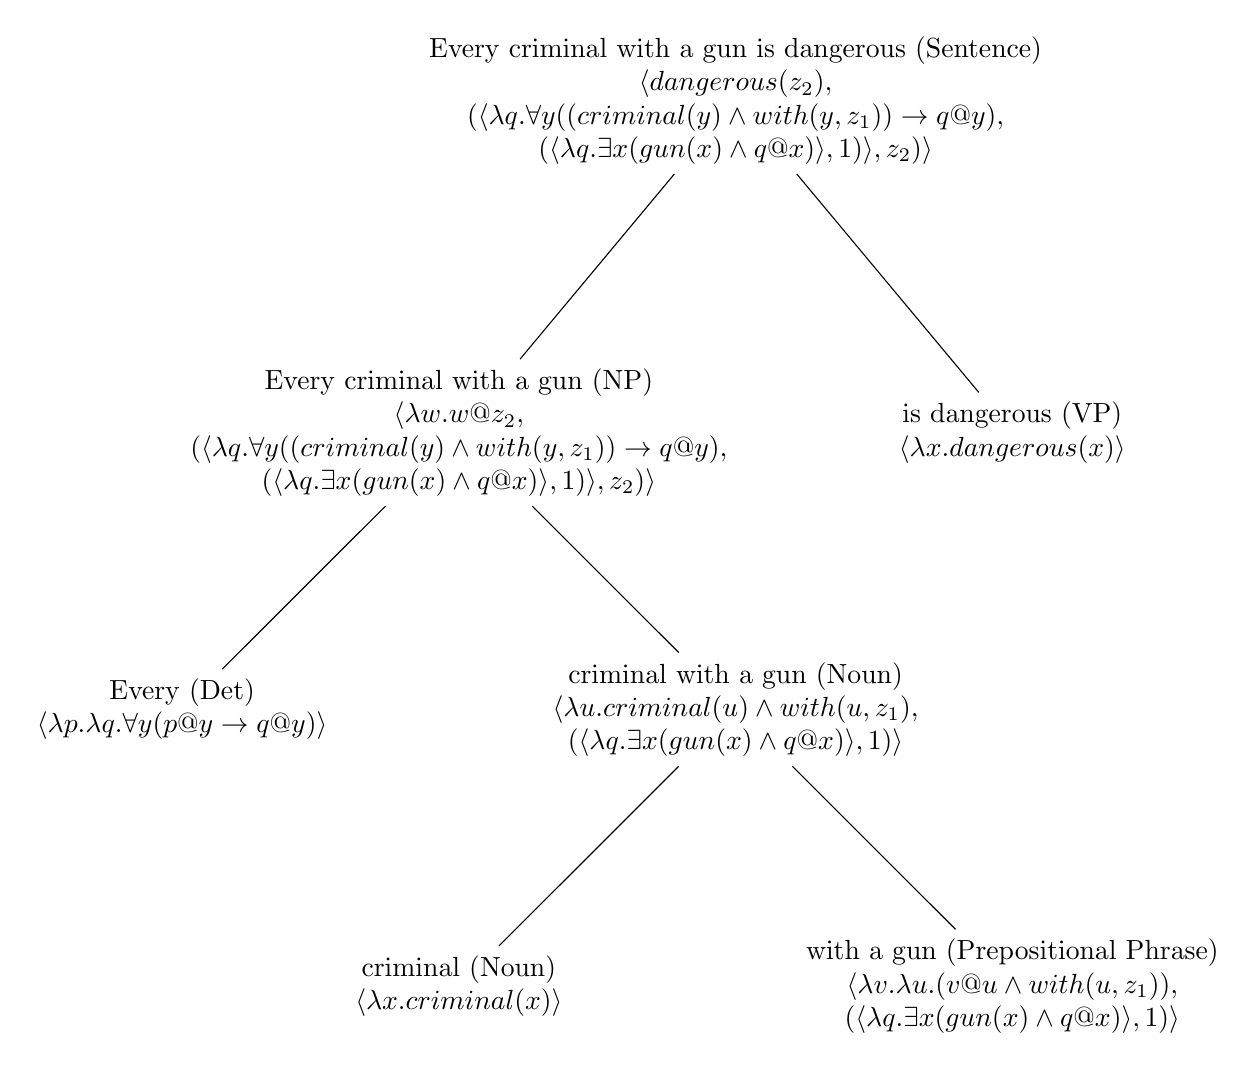
\begin{tikzpicture}[align = center, sibling distance = 200pt, level distance = 120pt]
\tikzset{level 2/.style = {level distance = 100pt}}

\node {\teng{Every criminal with a gun is dangerous} (\teng{Sentence}) \\ $\langle dangerous(z_2),$\\$(\langle \lambda q. \forall y((criminal(y) \land with(y,z_1)) \rightarrow q@y),$\\$ (\langle \lambda q. \exists x(gun(x) \land q@x) \rangle, 1) \rangle, z_2) \rangle$}
 child {node {\teng{Every criminal with a gun} (\teng{NP}) \\ $\langle \lambda w. w@z_2,$\\$(\langle \lambda q. \forall y((criminal(y) \land with(y,z_1)) \rightarrow q@y),$\\$ (\langle \lambda q. \exists x(gun(x) \land q@x) \rangle, 1) \rangle, z_2) \rangle$ }
  child {node {\teng{Every} (\teng{Det}) \\ $\langle \lambda p. \lambda q. \forall y(p@y \rightarrow q@y) \rangle$ }}
  child {node {\teng{criminal with a gun} (\teng{Noun}) \\ $\langle \lambda u. criminal(u) \land with(u,z_1),$\\$(\langle \lambda q. \exists x(gun(x) \land q@x) \rangle, 1) \rangle$ }
   child {node {\teng{criminal} (\teng{Noun}) \\ $\langle \lambda x. criminal(x) \rangle$}}
   child {node {\teng{with a gun} (\teng{Prepositional Phrase}) \\ $\langle \lambda v. \lambda u. (v@u \land with(u,z_1)),$\\$ (\langle \lambda q. \exists x(gun(x) \land q@x) \rangle, 1) \rangle$}}} }
 child {node {\teng{is dangerous} (\teng{VP}) \\ $\langle \lambda x.dangerous(x) \rangle$ }};
 
%\Tree [.NP [.Adj tall ] [.N tree ] ]
%\Tree [\node{aa} child {node {bb}} child [.cc d]; [.Adj C ] [.N E ] ]
\end{tikzpicture}
\end{center}
\caption{Semântica de Cooper}
\label{tree:keller}
\end{figure}

Agora, realizando a extração, podemos fazê-la apenas de um modo: $\exists x(gun(x) \land \forall y((criminal(y) \land with(y,x)) \rightarrow dangerous(y)))$. Isto é a interpretação correta, não tendo sido gerado nenhum problema. As outras opções de (não-)extração funcionam de modo semelhante.

Assim, o problema dos sintagmas nominais é resolvido. Apesar disso, o segundo problema apontado, do escopo das negações, persiste. As interpretações geradas são as mesmas de antes, pelo armazenamento de Cooper.  Portanto, o método de Keller aprimora os resultados de Cooper, sem resolver todas os obstáculos gerados por ambigüidades de escopo.

\subsection{\teng{Hole Semantics}}

Apesar de ser possível criar um novo mecanismo para capturar a ambigüidade de escopo gerada pela negação\footnote{Com efeito, em nosso repositório apresentamos no arquivo \textsc{negationKellerStorage.pl} uma alteração neste sentido. \todo[inline,color=yellow]{atualizado}}, abordagens \textit{ad hoc} para novas dificuldades fere a extensibilidade da gramática, criando uma falta de harmonização dos métodos usados, possivelmente proliferando uma diversidade de construções muito distintas entre si. Se possível, desse modo, precisamos de uma abordagem mais uniforme. Na realidade, não apenas a negação traz ambigüidades de escopo. Por exemplo, uma frase como \expreng{If a man walks then he jumps and a woman is happy} é ambígua \citep{HoleSem}. Podemos imaginar uma interpretação na qual \expreng{a woman is happy} é parte do conseqüente da implicação e outra na qual não o é, sendo uma afirmação separada da implicação.\footnote{Este tipo de construção não ocorre no programa original de \citet{BlackburnBos:2005}, por não haver orações coordenadas com \expreng{and}, nem coordenação com orações já coordenadas com outras. O código foi modificado para que isso fosse}\todo{AJUSTAR - ambigüidade semântica ou sintática?} Em razão destas dificuldades, e também de modo a ganhar maior flexibilidade na representação, analisaremos uma outra forma de representação semântica, não baseada em armazenamentos. 

Assim como nos métodos baseados em armazenamentos, uma frase não será associada uma expressão de primeira ordem, mas a uma representação abstrata, que então é associada a um conjunto de expressões em primeira ordem. Entretanto, o modo pelo qual isso é feito aqui é distinto. Em \teng{Hole Semantics}, uma idéia essencial é a de \textit{restrições}: podemos pensar na representação como um conjunto de restrições, de modo que qualquer fórmula de primeira ordem que satisfaça as restrições será uma interpretação possível para a frase \cite[p.~129]{BlackburnBos:2005}. A representação será referida por representação subespecificada (\teng{USR}, de \teng{underspecified representation}).

Uma fórmula de primeira ordem possui uma decomposição única como uma árvore, em razão pelo modo como é montada. Por exemplo, para a frase \expreng{If Mia loves John then Mia does not hurt John} tem associada à sua semântica a fórmula $love(mia,john) \rightarrow (\neg hurt(mia,john))$, que pode ser decomposta na árvore:

\begin{center}
\begin{tikzpicture}[sibling distance=25mm]
\node {$\rightarrow$}
 child {node {$love(mia,john)$}}
 child {node {$\neg$}
  child {node {$hurt(mia,john)$}}};
\end{tikzpicture}
\end{center}

As restrições serão sobre o modo de construir a fórmula. Dito de outro modo, a USR será um modo de falar a respeito da árvore de cada interpretação possível. Ao invés de montarmos uma única árvore (o que corresponderia a uma única fórmula), a USR pode ser pensada como uma ``árvore incompleta'', isto é, uma árvore com ``buracos'', justificando o nome desse método. Entretanto, estes buracos não poderão ser preenchidos de qualquer modo, havendo relações de \textit{dominância}. Um buraco deverá dominar um nó quando estiver acima do mesmo na representação da árvore. A partir daí, as subfórmulas irão compôr a fórmula completa através de um ``preenchimento'' dos buracos. Este ``preenchimento'' será feito \textit{encaixando} algum nó (junto com sua sub-árvore) no buraco.

Nos métodos de armazenamentos, a semântica das frases era representada por um vetor que continha um núcleo e os quantificadores guardados em (um aninhamento de) operadores de ligação. Em \teng{Hole Semantics}, nosso modo de representar será bem distinto. Na realidade, nós usaremos uma linguagem lógica para essa representação, chamada \textit{linguagem de representação subespecificada} (\teng{URL}, do inglês \teng{underspecified representation language}). A linguagem original, que aqui é alguma forma de lógica de primeira ordem, será referida por \textit{linguagem de representação semântica} (\teng{SRL}, \teng{semantic representation language}). Pode causar algum espanto o fato de que a URL será, ela própria, uma linguagem de primeira ordem! Seu vocabulário será definido do seguinte modo:

\begin{enumerate}
\item Predicados binários $\textsc{:not}$ e $\leq$
\item Predicados ternários $\textsc{:imp}$, $\textsc{:and}$, $\textsc{:or}$, $\textsc{:all}$, $\textsc{:some}$ e $\textsc{:eq}$
\item Cada constante no vocabulário da SRL também é uma constante no vocabulário da URL.
\item Para cada predicado $n$-ário $pred$ na SRL, $\textsc{:pred}$ é um predicado $(n+1)$-ário na URL.
\end{enumerate}

A lógica de primeira ordem utilizada é \textit{tipada}, havendo três tipos. O primeiro deles é o dos \textit{buracos}, cujas variáveis serão denotadas por $h$, $h'$, $h_1$, $h_2$, etc. O segundo é o tipo dos \textit{rótulos}, cujas variáveis são escritas $l$, $l'$, $l_1$, etc. Cada rótulo marcará um vértice na árvore que não é um buraco, sendo um modo de se referir aos símbolos da SRL. Por fim, o terceiro tipo é o das \textit{meta-variáveis}, escritos $v$, $v'$, $v_1$, $v_2$, etc. As meta-variáveis têm a função de se referir às variáveis da SRL.

Dizemos que algo é um \textit{nó} se for um buraco ou um rótulo. Dizemos que algo é um \textit{meta-termo} da URL caso seja uma \textit{meta-variável} ou uma constante da URL.

Agora, iremos definir as USRs básicas:

%\begin{defn}[USR básica] \leavevmode
\begin{enumerate}
\item Se $l$ é um rótulo e $h$ é um buraco, então $l \leq h$ é uma USR básica. \label{om-const}
\item Se $l$ é um rótulo e $n$ e $n'$ são nós, então $l\textsc{:not}(n)$, $l\textsc{:imp}(n,n')$, $l\textsc{:and}(n,n')$ e $l\textsc{:or}(n,n')$ são USRs básicas.
\item Se $l$ é um rótulo enquanto $t$ e $t'$ são meta-termos, então $l\textsc{:eq}(t,t')$ é uma USR básica.
\item Se $l$ é um rótulo, $S$ é um símbolo $n$-ário na linguagem SRL e $t_1$, \dots, $t_n$ são meta-termos, então $l\textsc{:S}(t_1,\dots, t_n)$ é uma USR básica.
\item Se $l$ é um rótulo, $v$ é uma meta-variável, $n$ é um nó,	então $l\textsc{:some}(v,n)$ e $l\textsc{:all}(v,n)$ são USR básicas.
\item Nada mais é uma USR.
\end{enumerate}
%\end{defn}

Observe aqui que o espaço a mais criado pela subida de aridade nos predicados e conectivos é preenchido pela variáveis de rótulo. Observe que o item \ref{dom-const} é o único que utiliza o símbolo de $\leq$. USRs básicas desta forma são ditas \textit{restrições de dominância}. Por fim, podemos definir o restante das USRs:

%\begin{defn}[USR]\leavevmode
\begin{enumerate}
\item Toda USR básica é uma USR.
\item Se $\phi$ é uma USR e $n$ é um nó, então $\exists n \phi$ é uma USR.
\item Se $\phi$ é uma USR e $v$ é uma meta-variável, então $\exists v \phi$ é uma USR.
\item se $\phi$ e $\psi$ são USRs, então $\phi \land \psi$ é uma USR.
\item Nada mais é uma USR.
\end{enumerate}
%\end{defn}

É de ser notado que nem todos os conectivos e formas da lógica da primeira ordem foram empregados nesta definição. Na realidade, apenas são fórmulas conjuntos pequenos de formas conjuntivas e existencialmente fechadas. Entretanto, esse fragmento da linguagem é suficiente para nossos propósitos \citep[p.~131]{BlackburnBos:2005}.

Podemos avançar então para um exemplo. Consideremos a frase \expreng{Mia does not love a man}. Uma interpretação é aquela na qual Mia não ama um homem específico, que pode ser formalizada como $\exists x: man(x) \land \neg love(mia,x)$. Outra, é aquela na qual Mia não ama homem algum, isto é, $\neg (\exists x: man(x) \land love(mia,x))$. Suas árvores são:

\begin{center}
\begin{tikzpicture}[sibling distance=25mm]
\node at (-4,0) {$\exists x$}
 child {node {$\land$}
  child {node {$man(x)$}}
  child {node {$\neg$}
   child {node {$love(mia,x)$}}}};

\node at (4,0) {$\neg$}
 child {node {$\exists x$}
  child {node {$\land$}
   child {node {$man(x)$}}
   child {node {$love(mia,x)$}}}};
\end{tikzpicture}
\end{center}

Já a representação subespecificada busca capturar o que há em comum entre as árvores possíveis. A USR desta frase é: 

\begin{flalign*}
&\exists h_0 \exists h_1 \exists h_2 \exists l_1 \exists l_2 \exists l_3 \exists l_4 \exists l_5 \exists v_1 \\& ({l_1\textsc{:not}(h_1)} \land l_2\textsc{:love}(mia,v_1) \land l_3\textsc{:some}(v_1,l_4) \land l_4\textsc{:and}(l_5, h_2) \land l_5\textsc{:man}(v_1))
\end{flalign*}

Porém, as USRs se tornam melhor compreensíveis através de sua representação gráfica, estando abaixo aquela relativa à nossa frase considerada:

\begin{center}
\begin{tikzpicture}
[node distance = 3cm, auto, thick, inner sep=2mm, def/.style={circle,draw}]

\node (h0) at ( 0,0)  {$h_0$};
\node (l1) at ( 2,-2) {$l_1: \neg h_1$} edge [dotted] (h0);
\node (h1) at (2.3,-2) {};
\node (l2) at ( 2,-4) {$l_2: love(mia, v_1)$} edge [dotted] (h1);
\node (l3) at ( -3,-2) {$l_3: \exists v_1(l_4)$} edge [dotted] (h0);
\node (l4ref) at (-2.2,-2) {};
\node (l4) at (-3,-3) {$l_4: l_5 \land h_2$} edge [<-] (l4ref);
\node (l5ref) at (-3,-3.1) {};
\node (h2) at (-2.3,-3) {} edge [dotted] (l2);
\node (l5) at (-5,-4) {$l_5: man(v_1)$} edge [<-] (l5ref);


%\draw [<->] (dir) to (ob/3);
%\draw [->] (ob/2) to (lib);
%
%\end{tikzpicture}
%\end{center}

\end{tikzpicture}
\end{center}


Podemos ver a intuição desta representação. É criado um buraco $h_0$ correspondente ao nó mais alto da árvore. As linhas pontilhadas representam restrições de dominância entre buracos e nós. Por sua vez, as linhas preenchidas mostram quais nós são pais de outros. A relação de parentesco também representa dominância: se um nó é pai de outro, é certo que o filho não pode ter escopo mais externo que o pai, uma vez que deve ser subfórmula do mesmo. Entretanto, neste caso a posição está fixa: necessariamente a relação de parentesco será aquela. Por sua vez, na dominância entre buracos e nós, não é isto que occore. Basta que o nó dominado esteja no escopo do nó dominante, não necessariamente sendo filho do mesmo. Ou seja, basta ser descendente.

Agora, a nossa análise de frases é feita ainda decompondo sintaticamente, e então, para cada termo, criando uma representação na forma de uma USR. Ainda utilizamos o cálculo lambda para fazer combinações de expressões. A representação final da frase é feita por combinações das representações das partes que as constituem. Por exemplo, a representação para o determinante \expreng{a} é:

\begin{flalign*}
	& \lambda x. \lambda y. \lambda h. \lambda l. \exists h_1 \exists l_1 \exists l_2 \exists l_3 \exists v_1 \\& (l2\textsc{:all}(v_1,l_3, \land l3 \textsc{:and}(l_1,h_1) \land l \leq h_1 \land l_2 \leq h \land x@v_1@h@l_1 \land y@v_1@h@l))
\end{flalign*}

Por sua vez, para o substantivo \expreng{woman} é:
\begin{flalign*}
\lambda v. \lambda h. \lambda l. (l\textsc{:woman}(v) \land l \leq h  )&&
\end{flalign*}

Assim, o sintagma nominal $\expreng{a woman}$ fica, aplicando a segunda representação na primeira e beta-reduzindo:
\begin{flalign*}
&\lambda y. \lambda h. \lambda l. \exists h_1 \exists l_1 \exists l_2 \exists l_3 \exists v_1 \\& (l2\textsc{:all}(v_1,l_3, \land l3 \textsc{:and}(l_1,h_1) \land l \leq h_1 \land l_2 \leq h \land l_1\textsc{:woman}(v_1) \land l_1 \leq h \land y@v_1@h@l))
\end{flalign*}

Definindo as USRs para cada função sintática e o modo de combiná-las, obtemos a USR da frase. Com isto em mãos, precisamos ser capazes de construir as árvores possíveis. Isso é feito por meio de \textit{encaixes}\footnote{Em inglês, o termo usado é \expreng{plug}, por isso a letra utilizada é $P$.}. Para cada buraco, achamos um rótulo candidato para preenchê-lo: este rótulo será encaixado no buraco. Mais formalmente, um encaixe é uma função injetiva dos buracos aos rótulos. Entretanto, nem todo encaixe nos satisfaz. Evidentemente, queremos satisfazer duas condições: queremos que o resultados seja uma árvore (portanto, acíclica e conexa), bem como queremos que, se existe uma restrição de dominância de um buraco $H$ sobre um rótulo $L$ (ou seja, se $L \leq H$), então $L$ será descendente de $H$ na árvore.

Para o exemplo que vimos, dois encaixes são possíveis: $P_1(h_0) = l_1, P_1(h_1) = l_3, P_1(h_2) = l_2$ e $P_2(h_0) = l_3, P_2(h_1) = l_2, P_2(h_2) = l_1$.

Assim, duas árvores são formadas, cada uma gerando uma interpretação possível. Pelo encaixe $P_1$ obtemos a árvore \ref{tree:p1}. Já pelo $P_2$, temos a árvore \ref{tree:p2}.

\begin{figure}[h]
\begin{center}
\begin{tikzpicture}[sibling distance=50mm]
\node {{$h_0$}}
  child {node {$l_1: \neg h_1$}
   child {node {$l_3: \exists v_1(l_4)$}
    child {node {$l_4: l_5 \land h_2$}
     child {node {$l_5: man(v_1)$}}
     child {node {$l_2: love(mia,v_1)$}}}}};
\end{tikzpicture}
\end{center}
\caption{$P_1$}
\label{tree:p1}
\end{figure}

\begin{figure}[h]
\begin{center}
\begin{tikzpicture}[sibling distance = 50mm]
\node {{$h_0$}}
 child {node {$l_3: \exists v_1(l_4)$}
  child {node {$l_4: l_5 \land h_2$}
   child {node {$l_5: man(v_1)$}}
   child {node {$l_1: \neg h_1$}
    child {node {$l_2: love(mia,v_1)$}}}}};
\end{tikzpicture}
\end{center}
\caption{$P_2$}
\label{tree:p2}
\end{figure}

Com efeito, estas são de fato as árvores que havíamos construído antes, para cada interpretação.

\todo[color=Green,inline]{Grafos e árvores colocados como figures flutuantes.}
